\chapter{The Norwegian Young Sea Ice Field Expedition}



 The research vessel R/V Lance was frozen into first-year sea ice in the Atlantic sector of the Arctic ocean and drifted with the sea ice. Three times during the expedition the ice surrounding the ship broke up and the ship needed to be repositioned into the sea ice. The time it took for the ship to reposition can be seen as gaps in the data from 21 February, through 24 February, 15 March through 24 April, and again from 5 June through 7 June. Note that the period in March and April corresponds with a trip back to Svalbard for resupply, explaining the long duration of the data gap.

This expedition is of particular interest from a modeling perspective due to the magnitude of the temperature and pressure change during and after winter storm periods. This research cruise is the first to take measurements of the clouds and atmosphere since the Surface Heat Budget of the Arctic (SHEBA) field experiment in 1997 and 1998. However, the storms observed during the N-ICE2015 observational period showed temperature increases significantly larger than those seen at SHEBA \citep{cohen:2017}. Additionally, throughout much of the expedition, strong temperature inversions were observed over the surface, similar to what was seen at SHEBA \citep{kayser:2017}. While these strong inversions are not unique to N-ICE2015, they are often underrepresented in Polar WRF simulations \citep{hines:2015}.

\section{Introduction}

N-ICE 2015 was a 6-month field experiment spanning from January to July 2015, observing both atmospheric properties and ice dynamics. A research icebreaker vessel, the RV Lance, was frozen into the sea ice north of Svalbard and allowed to move with the ice floes. The ship tracks can be seen in \ref{fig:ch1_f1}. This location sees thin, first-year sea ice, as opposed to the thick, multi-year sea ice observed during SHEBA \citep{cohen:2017}. As a result, N-ICE is representative of the new regime that the polar regions are moving toward as the climate warms. 

The primary objectives of N-ICE are:

\begin{enumerate}
    \item To quantify the change in atmosphere-ice-ocean interactions as the atmosphere shifts from primarily multi-year sea ice to thin, first-year sea ice \citep{granskog:2018, granskog:2015}. 
    \item Observe how changes in sea ice impact the marine ecosystem and their response \citep{granskog:2015}.
    \item Provide key observations to tune and validate global circulation models \citep{granskog:2018, granskog:2015}.
\end{enumerate}

\section{Experiment Description}

Measurements of the energy balance and cloud properties (fraction, height, microphysical, and temperature) can give important insight into climate processes and radiative transfer but are rarely measured together \citep{persson:2002, schweiger:2004}. The Norwegian Young Sea Ice Experiment (N-ICE2015) is the first experiment to study all of these factors during both winter and summer since SHEBA in 1997 and 1998 \citep{walden:2017}. 

There were several periods of low atmospheric pressure and increased wind speed that were defined as storms. These storms were also accompanied by increases in the integrated water vapor and changes in wind direction \citep{kayser:2017}. Storms are further described in \citet{cohen:2017, kayser:2017}. More details about the experiment and datasets collected can be found in \citet{granskog:2015}. There are three gaps in the dataset resulting from the ice breakup. During the experiment, the floe that the ship was anchored to broke apart, resulting in the inability to continue measurements on  the surrounding sea ice. During these times, the instruments were removed from the sea ice, and the ship then sailed to another floe further north on which the instruments were redeployed. \citet{itkin:2017} describes the proximity to the sea ice edge throughout the experiment. During the majority of the experiment, the ship was stationed between 50 and 250 $km$ from the ice edge. 

\begin{figure}[H]
    \centering
    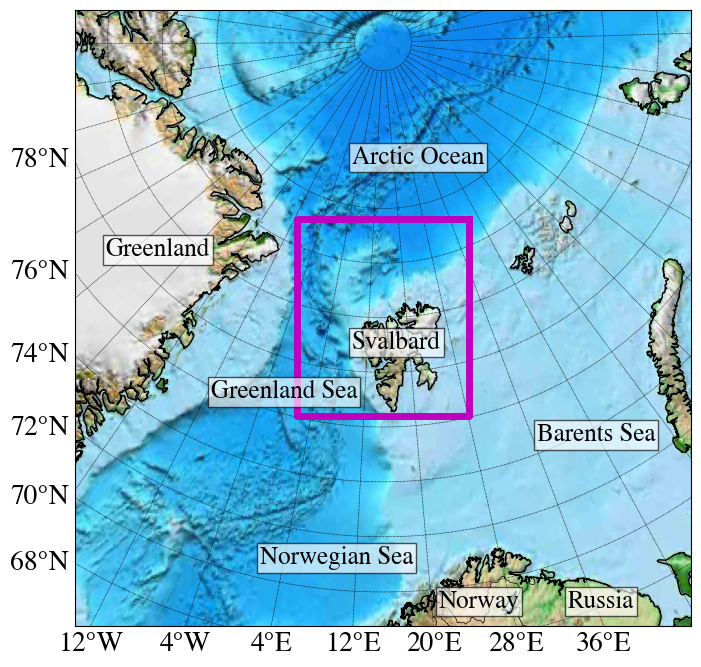
\includegraphics[width=0.5\linewidth]{figures/chapter2/ship_zoom_out.png}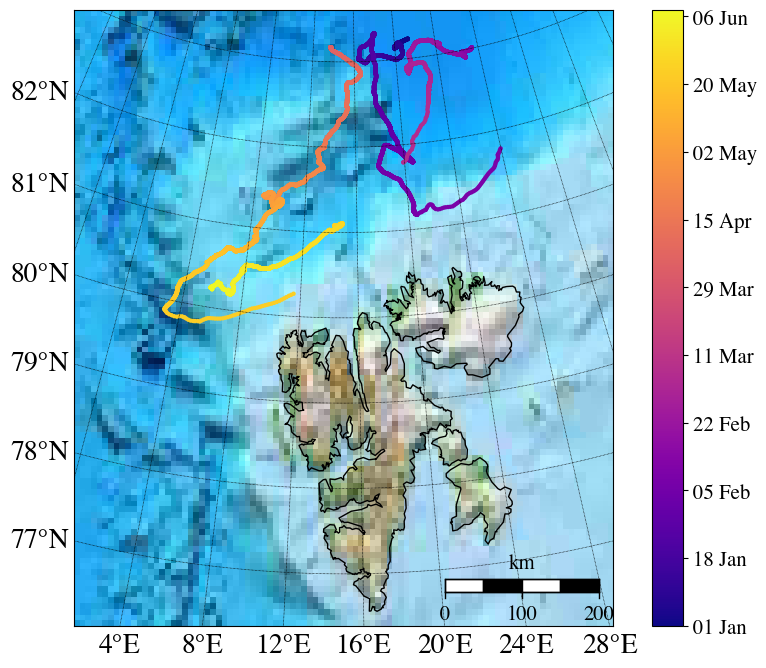
\includegraphics[width=0.55\linewidth]{figures/chapter2/ship_zoom_in.png}
    \caption[N-ICE location.]{The location of the N-ICE field expedition. The right figure shows a detailed view of the area in the purple box on the left map. Ship location is plotted on the right figure and is colored by date.}
    \label{fig:nice}
\end{figure}


\begin{table}[H]
\centering
\footnotesize
{
\begin{tabular}{| c | c | c |}
 \hline
\rowcolor[HTML]{F3F3F3} \textbf{Floe} & \textbf{Start Date} & \textbf{End Date} \\
  \hline
 1 & 15 January 2015 & 21 February 2015 \\
 2 & 24 February 2015 & 19 March 2015 \\ 
 3 & 18 April 2015 & 5 June 2015\\
 4 & 7 June 2015 & 21 June 2015 \\
  \hline
\end{tabular}}
\caption{Floe does for the N-ICE field expedition.}
\label{tab:floedates}
\end{table}



A variety of instruments were deployed during the N-ICE campaign that will be used in this project, including  radiosondes, a MicroPulse Lidar (MPL), a meteorological tower, an Eddy Covariance system, and broadband shortwave and longwave radiometers. 

Vaisala RS92-SGP radiosondes were launched from the ice surface (first Floe) or the ship deck (following three floes) twice daily around 1100 and 2300 UTC. They recorded temperature, relative humidity, wind speed and direction, pressure, and geopotential height as high as 30 $km$. Data are recorded by the radiosondes on a two-second time interval and transmitted to the ground using the Vaisala MW31 ground station \citep{kayser:2017, cohen:2017}. More information and analysis of the radiosondes can be found in \citet{kayser:2017}.

Data from the MPL were recorded every 14 seconds up to a height of 20 $km$. The MPL records backscattered light from clouds and operates at 532 $nm$. The range resolution is 15 m, with an 18 km maximum cloud base height. Signature distance uncertainties are $\pm$ 2 $\%$ due to timing uncertainties within the instrument. This instrument is more sensitive to water particles than ice, so some cloud types may be biased toward higher percentages of water than ice within the cloud. The MPL is easily attenuation by optically thick clouds. In some instances when a low water cloud is detected, it is possible that more cloud layers exist above this layer that can not be measured by the MPL. 

A meteorological tower was deployed on the ice 300 to 400 $m$ away from the ship. This tower was set up within a few days of anchoring to each new floe and recorded relative humidity and temperature (Vaisala HMP155), pressure (RM Young 61302 V), and wind speed and direction (Lufft Ventus V200A-UMB) at 2, 4, and 10 $m$ heights. All measurements were collected by a Campbell Scientific CR30000 data logger at 1-second resolution. Periods of missing tower data were reconstructed using temperature and wind information from the ship (sensors mounted 22 to 24 $m$ above the surface). More information about the meteorological measurements, temperature, and wind reconstruction using the ship data, a diagram of the meteorological tower setup, and a comparison of the meteorology to SHEBA can be found in \citet{cohen:2017}.

Radiometers (Kipp and Zonen CMP22 and CGR4) were set up 1 to 1.2 $m$ above the surface near the meteorological tower to measure upward and downward components of longwave and shortwave components of radiation. Kipp and Zonen CVF4 ventilation units were used to heat and ventilate the radiometers. More information about the radiometers and an analysis of the surface energy budget can be found in \citet{walden:2017}.

Turbulent flux data were collected by a closed path EC flux system (Campbell CPEC200) at a varying frequency (10 or 20 $Hz$). This system contains a sonic anemometer and a closed-path, infrared gas analyzer. These allow observation of the heat and moment exchanges and the water vapor and carbon dioxide mixing ratios, respectively. This system was set up next to the meteorological tower over a snow-covered surface. Further information about the EC Flux system can be found in \citet{walden:2017}.


\section{N-ICE vs SHEBA: Key Differences}
% N-ICE vs SHEBA
\citet{shupe:2004} observed mixed-phase clouds during SHEBA were consistent in temperature, liquid water path, and ice water content with previous studies over similar sea ice. The largest disagreement with previous experiments occurred during winter storm periods. NICE2015 observed more extreme storm periods than those seen at SHEBA, bringing wind speed, pressure, and temperature changes of previously unobserved magnitudes. 

\section{Atmospheric components of the surface energy budget over young sea ice: Results from the N-ICE2015 campaign, Walden et al. (2017)}

This paper detailed the turbulent and radiative fluxes over thin sea ice. Surface and atmospheric conditions were also covered. Snow albedo was around 0.85 in the winter and between 0.72 and 0.80 in the spring and summer. Stable stability was found in the winter, followed by unstable in the spring, and approximately neutral in the summer (once 0 $^{\circ} C$ skin temperature was reached). Negative average radiative and turbulent heat fluxes occurred in the winter, ranging between 40 to 0 $Wm^{-2}$. In the summer, positive values of as high as 60 $Wm^{-2}$ were recorded. Winter sensible heat flux ranged from 20 to 30 $Wm^{-2}$ and spring and summer from 0 to -20 $Wm^{-2}$. Positive values indicate flux into the surface.

My contribution to this publication was to fix several problems with the flux dataset collected during the N-ICE campaign and to process the data through the EddyPro software. The most restrictive data problem was the number of data gaps throughout 30-minute data files, which was caused by a programming error in the datalogger. In some cases, the amount of missing data made the file unable to be processed. To fix this, the data were filled by taking the section of data before it (or after, in the case that the missing data was too close to the start of the dataset) and replicating it for the time period with no recorded data. To ensure that this method of data filling was acceptable, data from Barrow, Alaska was used to compare the post-processed data of a complete dataset with the post-processed results from the same dataset after (artificially added) gaps had been filled. Analysis of both the difference in sensible heat fluxes and the turbulent spectra from before and after the data filling were examined and determined the filling method appropriate for the type of gaps in the N-ICE data. 